\documentclass{beamer}

\usepackage[utf8]{inputenc}
\usepackage[T1]{fontenc}

\usepackage{standalone}

\usepackage[acronym]{glossaries}

\usepackage{enumitem}

\usepackage{xcolor}

\usepackage{multirow}
\usepackage{multicol}

\usepackage{array}
\newcolumntype{x}[1]{>{\centering\let\newline\\\arraybackslash\hspace{0pt}}p{#1}}
\usepackage{booktabs}

\usepackage{siunitx}
\usepackage{mathrsfs, amsmath}

\usepackage{graphicx}
\usepackage[font={small, color=IGNDarkGrey}, labelformat=empty]{caption}
\usepackage{subcaption}
\DeclareCaptionFont{tiny}{\tiny}
\captionsetup[subtable]{labelfont={tiny, bf},textfont=normalfont,justification=raggedright}
\captionsetup[subfigure]{labelfont={tiny, bf},textfont=tiny,justification=raggedright}


\usepackage{hyperref}

\usepackage[
    mcite,
    backend=bibtex,
    style=verbose,
    citestyle=authoryear,
    bibstyle=numeric,
    sorting=none,
    autocite=footnote,
    maxnames=2,
    hyperref=true,
    natbib=true,
    abbreviate=true
]{biblatex}
\bibliography{references}
\setbeamerfont{footnote}{size=\tiny}


\usetheme{ign}


\newacronym{lod}{LoD}{Level of Detail}
\newacronym{lidar}{LiDAR}{Light Detection and Ranging}
\newacronym{dsm}{DSM}{Digital Surface Model}
\newacronym{gui}{GUI}{Graphical User Interface}

\title{Semantic $3D$ building model qualification}
\subtitle{}
\institute[LaSTIG MATIS]{Univ. Paris Est, LaSTIG MATIS, IGN, ENSG}
\date{\today}
\author[O.Ennafii]{Oussama Ennafii}

\begin{document}

    \begin{frame}[plain]
        \titlepage{}
    \end{frame}

    \section{Introduction}
        \subsection{Context}
            \begin{frame}{What is a $3D$ model?}
                \begin{itemize}[label=$\blacktriangleright$, font=\color{IGNGreen}]
                    \item<1-> $3D$ urban model $\equiv$ polyhedral surface modeling a building;
                    \item<2-> Holds higher semantic information than a $3D$ mesh while using less memory;
                \end{itemize}
                \uncover<3->{
                    \begin{figure}[H]
                        \begin{center}
                            
\includegraphics[height=.2\textheight]{images/citygml_lod}
                            \caption{\label{fig::lods_citygml} \gls{lod}~\footfullcite{kolbe2005citygml} representation as defined in the \emph{cityGML} format~\footfullcite{ohori2016higher}.}
                        \end{center}
                    \end{figure}
                }
            \end{frame}

            \begin{frame}{What is urban reconstruction?}
                \begin{itemize}[label=$\blacktriangleright$, font=\color{IGNGreen}]
                    \item<1-> The aim is to model urban objects, on a large scale, using:
                    \begin{itemize}[label=--]
                        \item<2-> unstructured data: \gls{lidar};
                        \item<3-> structured data: stereoscopic images.
                    \end{itemize}
                    \item<3-> The model \gls{lod} depends on:
                    \begin{itemize}[label=--]
                        \item<4-> their intended use,
                        \item<5-> the input data spatial resolution.
                    \end{itemize}
                \end{itemize}
            \end{frame}

            \begin{frame}{Urban models applications}
                \begin{itemize}[label=$\blacktriangleright$, font=\color{IGNGreen}]
                    \item<1-> Urban models have a wide application range~\footfullcite{Biljecki2015};
                \end{itemize}
                \uncover<2->{
                    \begin{table}
                        \begin{center}
                            \begin{tabular}{l l l}
                                \toprule
                                Planning & Simulation & Visualization \\
                                \midrule
                                City planning & Micro climates & Architecture \\
                                Emergency intervention & Wave propagation & Cadastre \\
                                Home decoration & Run-off water & Tourism \\
                                Communication network & Military intervention & Video games \\
                                \bottomrule
                            \end{tabular}
                            \caption{\label{tab::3d_applications} Some of the main thematic applications of $3D$ urban models.}
                        \end{center}
                    \end{table}
                }
            \end{frame}
        \subsection{Motivation}
            \begin{frame}{The need for self diagnostic}
                \begin{itemize}[label=$\blacktriangleright$, font=\color{IGNGreen}]
                    \item<1-> Automatic urban modeling is an active research area~\citep{Musialski2012}, but not \textcolor{IGNRed}{yet operational}~\citep{rottensteiner2014results}:
                    \begin{itemize}[label=--]
                        \item reconstruction methods lack generality and compacity;
                        \item too many modelling errors require labourious manual corrections.
                    \end{itemize}
                    \item<2-> Urban $3D$ model semantic diagnostic is not well studied~\citep{nguatem2017modeling}.
                \end{itemize}
                ~\\
                \uncover<3->{
                    \begin{itemize}[label=Goal $\longrightarrow$, font=\color{purple}, leftmargin=2cm]
                        \item Detect and describe semantic errors that affects building $3D$ models.
                    \end{itemize}
                }
            \end{frame}

            \begin{frame}{Potential use}
                \begin{itemize}[label=$\blacktriangleright$, font=\color{IGNGreen}, itemsep=2em]
                    \item<1-> Change detection;
                    \item<2-> Urban models correction;
                    \item<3-> Urban reconstruction method evaluation;
                    \item<4-> Crowd reconstruction quality assessment.
                \end{itemize}
            \end{frame}
    \section{State of the art}
        \begin{frame}{How to classify quality evaluation methods?}
            \begin{itemize}[
                    label=$\blacktriangleright$,
                    font=\color{IGNGreen},
                    itemsep=2em
                ]
                \item<1-> Based on the output:
                \begin{itemize}[label=--, itemsep=1em]
                    \item<2-> Geometric precision indices;
                    \item<2-> Semantic errors.
                \end{itemize}
                \item<3-> Based on the reference data:
                \begin{itemize}[label=--, itemsep=1em]
                    \item<4-> Manually obtained data;
                    \item<4-> Sensor data.
                \end{itemize}
            \end{itemize}
        \end{frame}
        \subsection{Different types of reference data}
            \begin{frame}{Manual data}
                Compare reconstructed $3D$ models with ground truth reference data with higher spatial accuracy, using:
                \begin{itemize}[label=$\blacktriangleright$, font=\color{IGNGreen}]
                    \item<1-> geodetic measurements ($ \sigma \sim \SI{0.05}{m}$)~\citep{Kaartinen2005, Voegtle2003};
                    \item<2-> stereo plotting~\citep{Kaartinen2005, Zeng2014}.
                \end{itemize}
                \uncover<3->{
                    Disadvantages:
                    \begin{itemize}[label=$-$, font=\color{IGNRed}]
                        \item<4-> too tedious to get.
                    \end{itemize}
                }
            \end{frame}

            \begin{frame}{Sensor data}
                Compare reconstructed $3D$ models with low semantic level sensor data, using:
                \begin{itemize}[label=$\blacktriangleright$, font=\color{IGNGreen}]
                    \item<1-> \gls{lidar}~\citep{Akca2010};
                    \item<2-> oriented aerial images~\citep{boudet2006supervised, Michelin2013}.
                \end{itemize}
                \uncover<3->{
                    Disadvantages:
                    \begin{itemize}[label=$-$, font=\color{IGNRed}]
                        \item<4-> no semantics.
                    \end{itemize}
                }
            \end{frame}
        \subsection{Different types of output}
            \begin{frame}{Geometric precision indices}
                Compute precision ratios from the $3D$ model which describes its quality.\\
                At different scales:
                \begin{itemize}[label=$\blacktriangleright$, font=\color{IGNGreen}]
                    \item<1-> Points of interest average precision~\citep{Kaartinen2005, Voegtle2003},
                    \item<2-> Surface discrepency to reference data~\citep{Kaartinen2005, Henricsson1997},
                    \item<3-> Volume discrepency to reference data~\citep{Zeng2014}.
                \end{itemize}
                \uncover<4->{
                    Disadvantages:
                    \begin{itemize}[label=$-$, font=\color{IGNRed}]
                        \item<5-> too general;
                        \item<6-> no semantics; thus no hierarchy.
                    \end{itemize}
                }
            \end{frame}

            \begin{frame}{Semantic errors}
                Identify the topologic and geometric errors that affects $3D$ models, using:
                \begin{itemize}[label=$\blacktriangleright$, font=\color{IGNGreen}]
                    \item<1-> visual inspection~\citep{OudeElberink2010};
                    \item<2-> supervized learning, detecting errors from a taxonomy based on:
                    \begin{itemize}[label=--]
                        \item<3-> traffic lights paradigm~\citep{boudet2006supervised};
                        \item<4-> a list of reconstruction errors~\citep{Michelin2013}.
                    \end{itemize}
                \end{itemize}
                \uncover<5->{
                    Risk:
                    \begin{itemize}[label=$-$, font=\color{IGNRed}]
                        \item<6-> overfitting to a scene or reconstruction method.
                    \end{itemize}
                }
            \end{frame}
        \subsection{Summary}
            \begin{frame}[plain]{Summary}
                \begin{figure}
                    \includegraphics[width=\textwidth]{state_of_the_art}
                    \caption{\label{fig::bib_summary} State of the art summary.}
                \end{figure}
            \end{frame}
            \begin{frame}{The ideal practical qualification paradigm}
                \begin{itemize}[label=$\blacktriangleright$, font=\color{IGNGreen}, itemsep=2em]
                    \item<1-> No reference data, or at least the most available sensor data;
                    \item<2-> Semantic errors.
                \end{itemize}
            \end{frame}
    \section{Methodology}
        \begin{frame}{How to predict reconstruction errors?}
            The problem is modeled as a supervised learning one based on an established error taxonomy:
            \begin{enumerate}[label = (\roman*)., font=\color{IGNGreen}]
                \item<2-> flexible: the error taxonomy is parametrizable;
                \item<3-> independent: the taxonomy is agnostic towards reconstruction methods;
                \item<4-> fast: does not involve heavy computing at runtime;
                \item<5-> modular: can use multiple entries:
                \begin{itemize}[label=--]
                    \item<6-> the model itself;
                    \item<7-> the corresponding \gls{dsm} (stereoscopic or \gls{lidar} based);
                    \item<8-> the corresponding orthoimage.
                \end{itemize}
                \item<9-> lightweight: does not involve manual reference data.
            \end{enumerate}
        \end{frame}
        \subsection{Pipeline}
            \begin{frame}{The Qualification pipeline}
                \begin{figure}
                    \includestandalone[mode=buildnew, width=1.05\textwidth]{pipeline}
                    \caption{\label{fig::pipeline} Pipeline describing the quality evaluation process.}
                \end{figure}
            \end{frame}
            \begin{frame}{The Qualification pipeline}
                \begin{itemize}[label=$\blacktriangleright$, font=\color{IGNGreen}]
                    \item<1-> Using \href{https://github.com/ethiy/proj.city}{\textcolor{IGNGreen}{proj.city}}, the first step extracts:
                    \begin{itemize}[label=--]
                        \item<2-> a facet adjacency graph from the model;
                        \item<2-> a $2D$ vector projection;
                        \item<2-> a $2D$ $z$ profile;
                    \end{itemize}
                    \item<3-> The second step extracts features from each representation of the model, with \href{https://github.com/ethiy/qualcity}{\textcolor{IGNGreen}{qualcity}}.
                    \item<4-> Using a \textcolor{IGNDarkOrange}{supervised classifer}, trained with the defined \textcolor{IGNDarkOrange}{taxonomy and parameters}, at the \textcolor{IGNDarkOrange}{building level}, we \textcolor{IGNDarkOrange}{predict} the building $3D$ model quality.
                \end{itemize}
            \end{frame}
        \subsection{Used Tools}
            \begin{frame}{\href{https://github.com/ethiy/proj.city}{proj.city}}
                This program was developped to:
                \begin{itemize}[label=$\blacktriangleright$, font=\color{IGNGreen}]
                    \item<1-> extracts models from urban scenes (\emph{3DS}, \emph{Obj}) at the building level;
                    \item<2-> computes the facet adjacency graph and some basic features (normal, area, centroid, degree, perimeter);
                    \item<3-> computes building model projection to $(O, \vec{i}, \vec{j})$ and store the result to a vector format (\emph{ESRI Shapefile}, \emph{GML}, \dots);
                    \item<4-> computes the model $z$ profile from the previous projection using the facets plane equations and save the result to a \emph{GeoTIFF}.
                \end{itemize}
            \end{frame}
            \begin{frame}{\href{https://github.com/ethiy/qualcity}{qualcity}}
                This program:
                \begin{itemize}[label=$\blacktriangleright$, font=\color{IGNGreen}]
                    \item<1-> reads and computes features from the previously saved representations;
                    \item<2-> retreives models labels;
                    \item<3-> infers the classification problem from the taxonomy parameters;
                    \item<3-> trains and tests the chosen classifier model.
                \end{itemize}
            \end{frame}
        \subsection{Error Taxonomy}
            \begin{frame}{Bidimensional taxonomy}
                In order to establish our taxonomy, two criterea are taken into account:
                \begin{itemize}[label=$\blacktriangleright$, font=\color{IGNGreen}]
                    \item<1-> the \acrfull{lod};
                    \item<2-> the \emph{finesse}: the semantization level.
                    \begin{itemize}
                        \item<3-> an error is of maximal \emph{finesse} $\Rightarrow$ corresponds to a unit (semantically) action required for the operator to correct the model: $\equiv$ \emph{atomic} error.
                    \end{itemize}
                \end{itemize}
            \end{frame}
            \begin{frame}{Taxonomy \emph{finesse}}
                \begin{enumerate}[label = (\roman*)., font=\color{IGNGreen}]
                    \item<1-> \emph{finesse} $0$ $\longrightarrow$ \textbf{Unqualifiable} / \textbf{Qualifiable};
                    \item<2-> \emph{finesse} $1$ $\longrightarrow$ \textbf{Valid} / \textbf{Erroneous};
                    \item<3-> \emph{finesse} $2$:
                    \begin{itemize}[leftmargin=12em, font=\color{IGNDarkOrange}]
                        \item[$\gls{lod}0 \cup \gls{lod}1 \longrightarrow$] \textbf{Building Errors}
                        \item[$\gls{lod}2 \longrightarrow$] \textbf{Facet Errors}
                        \item[$\gls{lod}3 \longrightarrow$] \textbf{Superstructure Errors}
                    \end{itemize}
                    \begin{figure}[H]
                        \begin{center}
                            
\includegraphics[height=.2\textheight]{images/citygml_lod}
                        \end{center}
                    \end{figure}
                    \item<4-> \emph{finesse} $3$ $\longrightarrow$ \emph{atomic} errors.
                \end{enumerate}

            \end{frame}
            \begin{frame}{\emph{Atomic} errors example}
                \only<1-5>{
                    For a \gls{lod} $ = 2$, we propose:
                    \begin{itemize}[label=$\blacktriangleright$, font=\color{IGNGreen}]
                        \item<1-> \textbf{Building Errors}:
                        \begin{itemize}[leftmargin=10em, font=\color{IGNDarkGreen}]
                            \item[Under segmentation:]<2-> two or more building reconstructed as one;
                            \item[Over segmentation:]<3-> one building subdivided into two or more buildings;
                            \item[Imprecise footprint:]<4-> inexact building footprint;
                            \item[Imprecise height:]<5-> inexact building height;
                        \end{itemize}
                    \end{itemize}
                }
                \only<6>{
                    \begin{figure}
                        \begin{center}
                            \begin{subfigure}{.28\textwidth}
                                \fbox{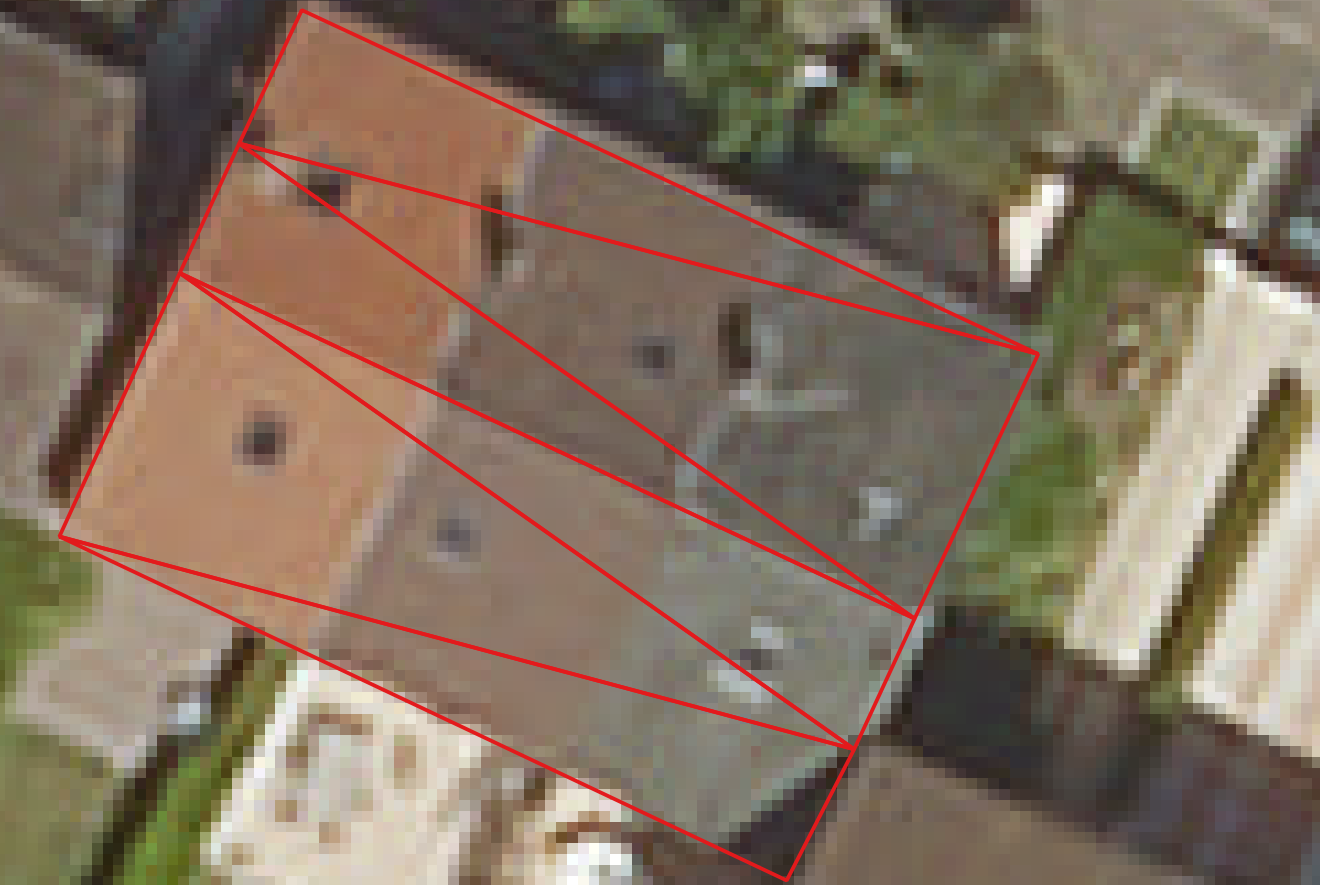
\includegraphics[width=\textwidth]{images/errors/building/under_segmentation}}
                                \caption{\label{fig::bul_under} Building under segmentation}
                            \end{subfigure}
                            \hspace{10pt}
                            \begin{subfigure}{.28\textwidth}
                                \fbox{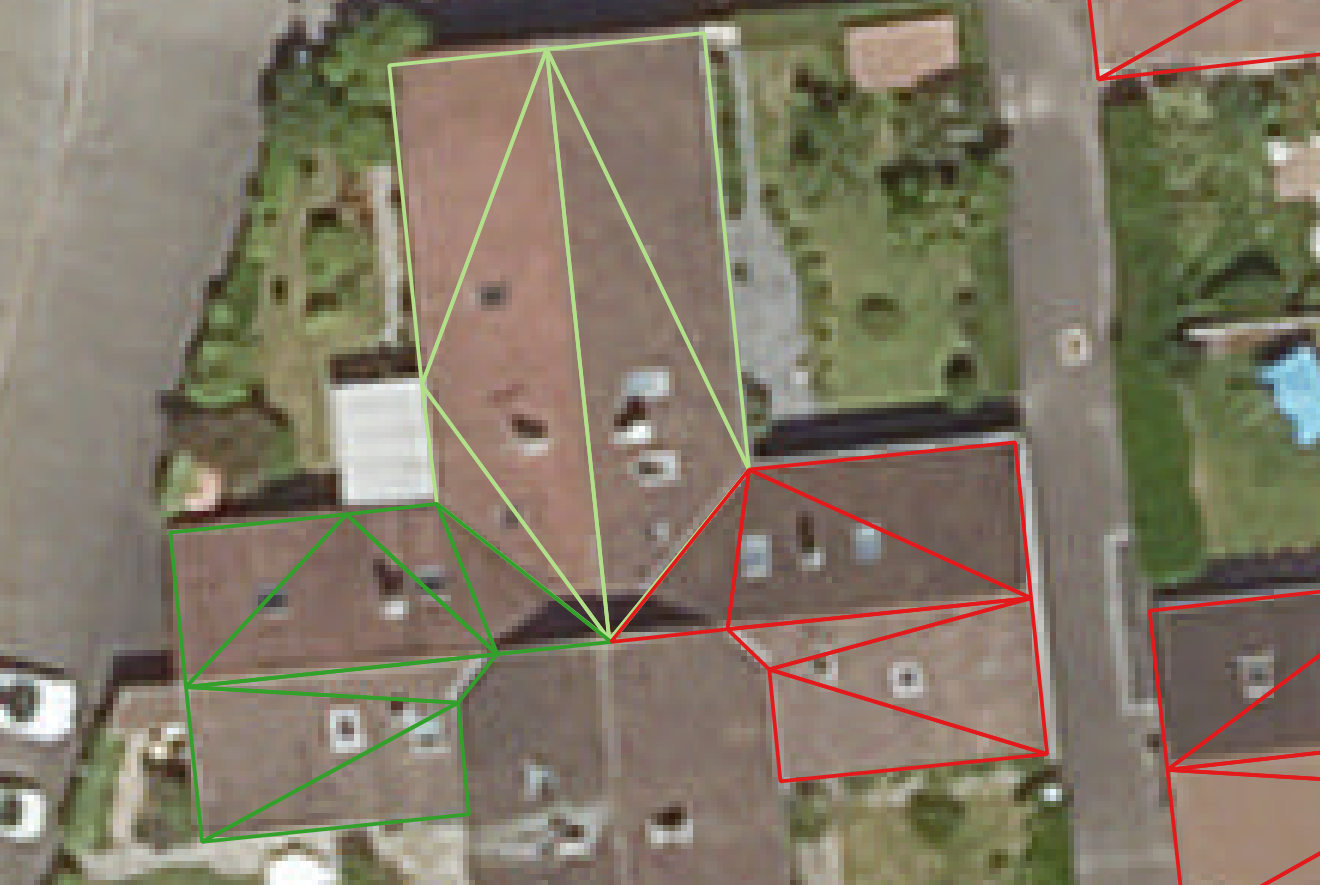
\includegraphics[width=\textwidth]{images/errors/building/over_segmentation}}
                                \caption{\label{fig::bul_over} Building over segmentation}
                            \end{subfigure}
                            \hspace{10pt}
                            \begin{subfigure}{.28\textwidth}
                                \fbox{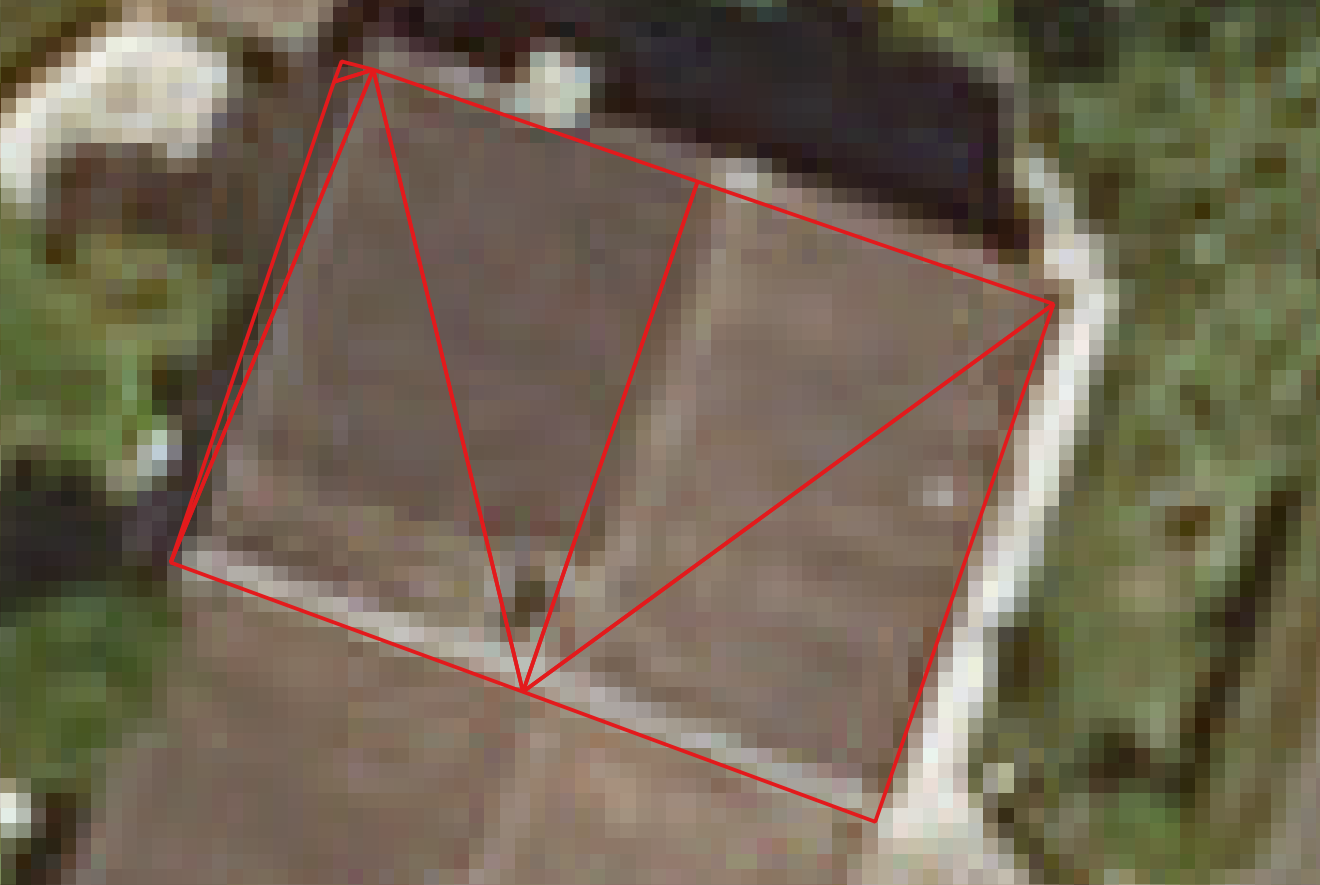
\includegraphics[width=\textwidth]{images/errors/building/footprint}}
                                \caption{\label{fig::bul_footprint} Imprecise footprint}
                            \end{subfigure}
                            \hspace{10pt}
                            \begin{subfigure}{.28\textwidth}
                                \fbox{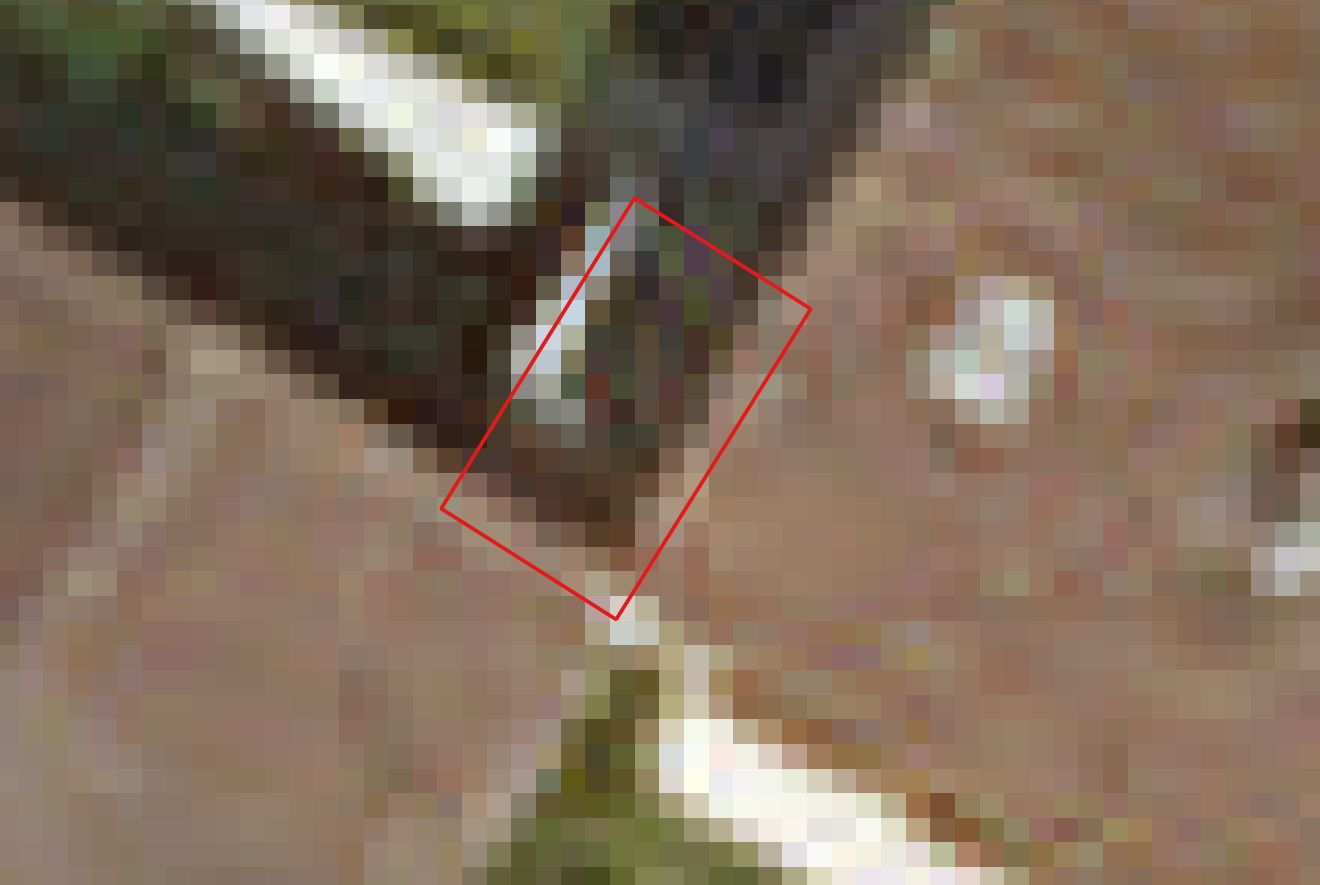
\includegraphics[width=\textwidth]{images/errors/building/altimetric}}
                                \caption{\label{fig::bul_height} Imprecise height}
                            \end{subfigure}
                            \caption{Building \emph{atomic} errors illustration.}
                        \end{center}
                    \end{figure}
                }
                \only<7-11>{
                    For a \gls{lod} $ = 2$, we propose:
                    \begin{itemize}[label=$\blacktriangleright$, font=\color{IGNGreen}]
                        \item<7-> \textbf{Facet Errors}:
                        \begin{itemize}[leftmargin=10em, font=\color{IGNDarkGreen}]
                            \item[Under segmentation:]<8-> two or more facets reconstructed as one;
                            \item[Over segmentation:]<9-> one facet subdivided into two or more facets;
                            \item[Imprecise Segmentation:]<10-> inexact edge betweeen facets;
                            \item[Imprecise slope:]<11-> inexact facet slope.
                        \end{itemize}
                    \end{itemize}
                }
                \only<12>{
                    \begin{figure}
                        \begin{center}
                            \begin{subfigure}{.28\textwidth}
                                \fbox{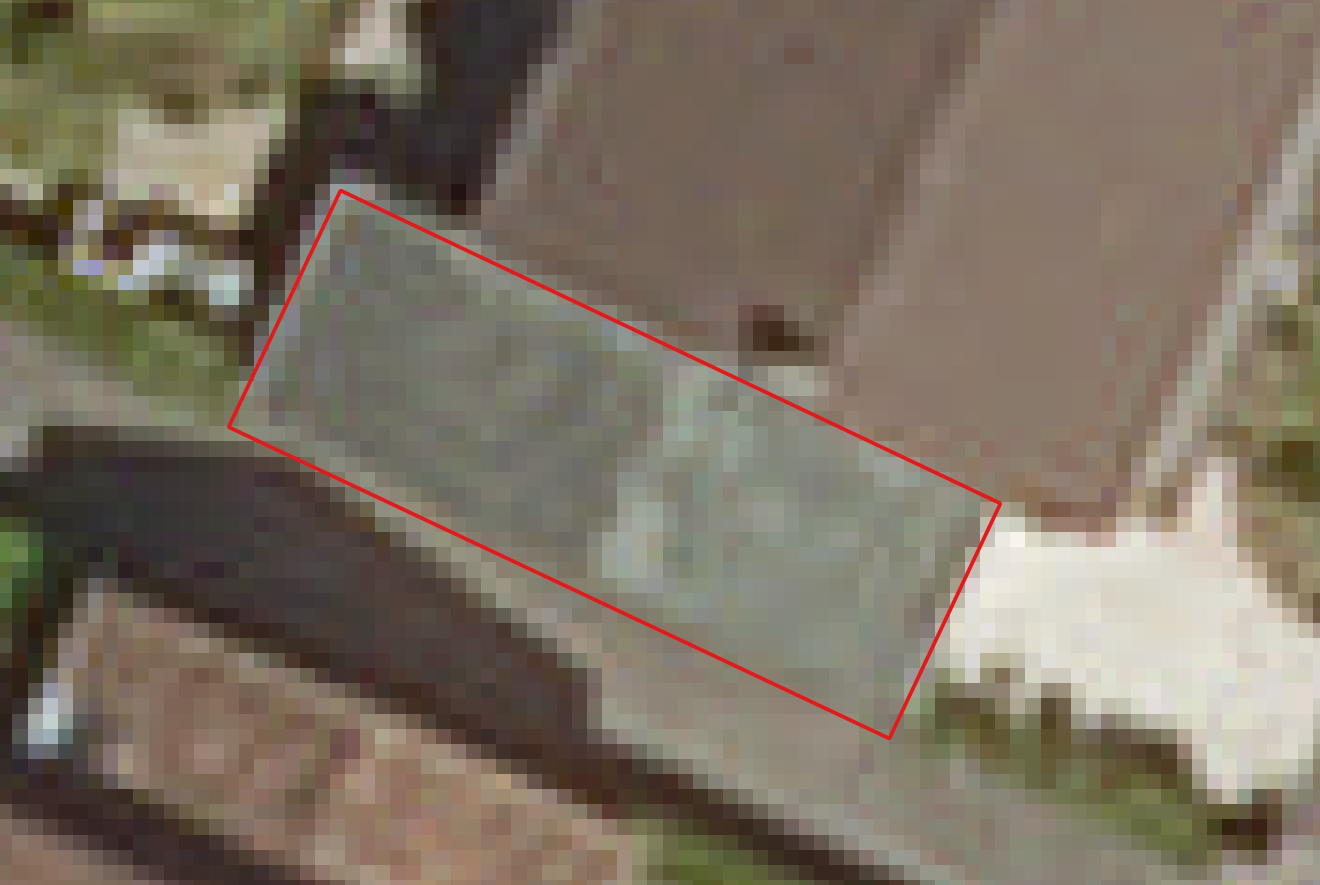
\includegraphics[width=\textwidth]{images/errors/facet/under_segmentation}}
                                \caption{\label{fig::fac_under} Facet under segmentation}
                            \end{subfigure}
                            \hspace{10pt}
                            \begin{subfigure}{.28\textwidth}
                                \fbox{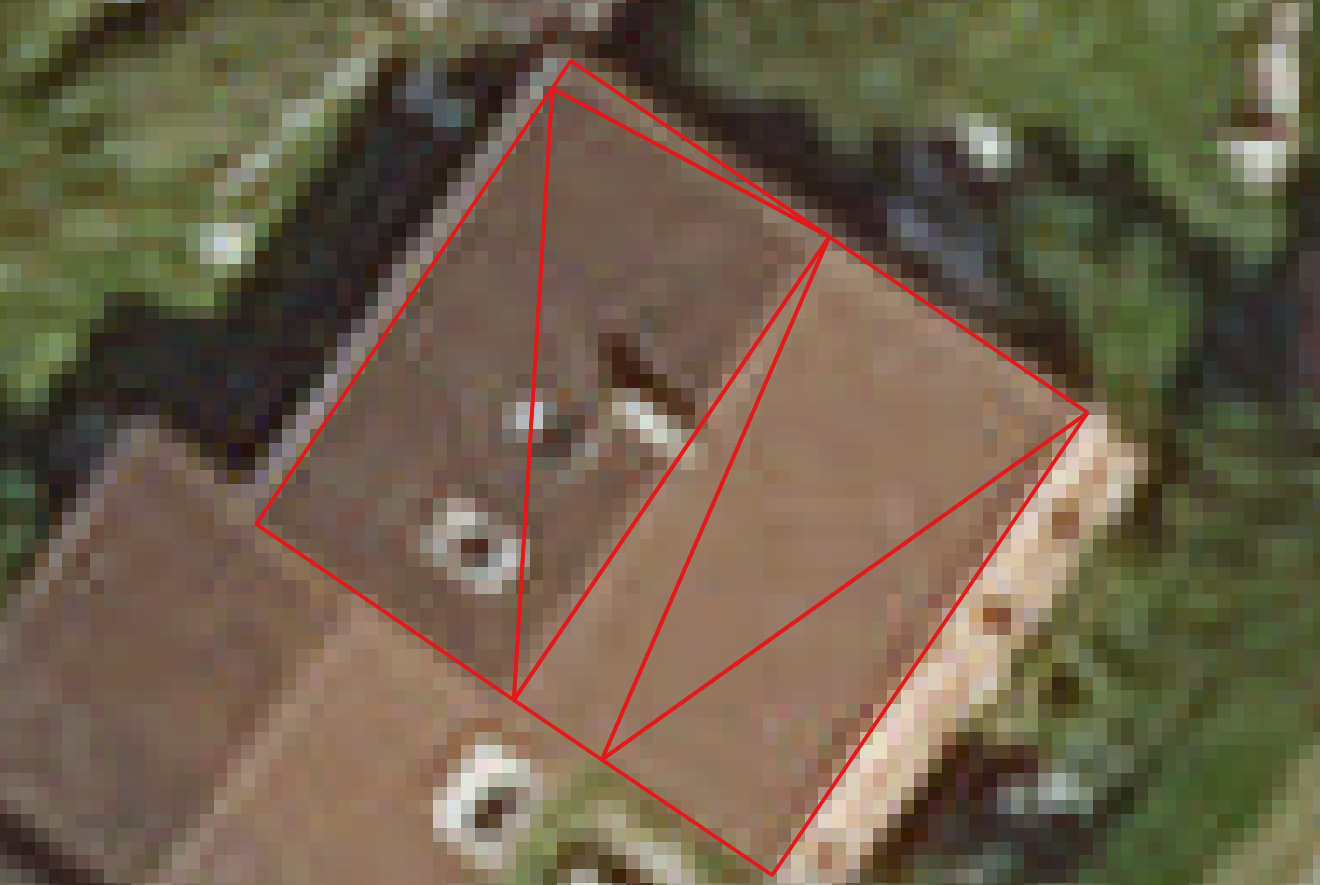
\includegraphics[width=\textwidth]{images/errors/facet/over_segmentation}}
                                \caption{\label{fig::fac_over} Facet over segmentation}
                            \end{subfigure}
                            \hspace{10pt}
                            \begin{subfigure}{.28\textwidth}
                                \fbox{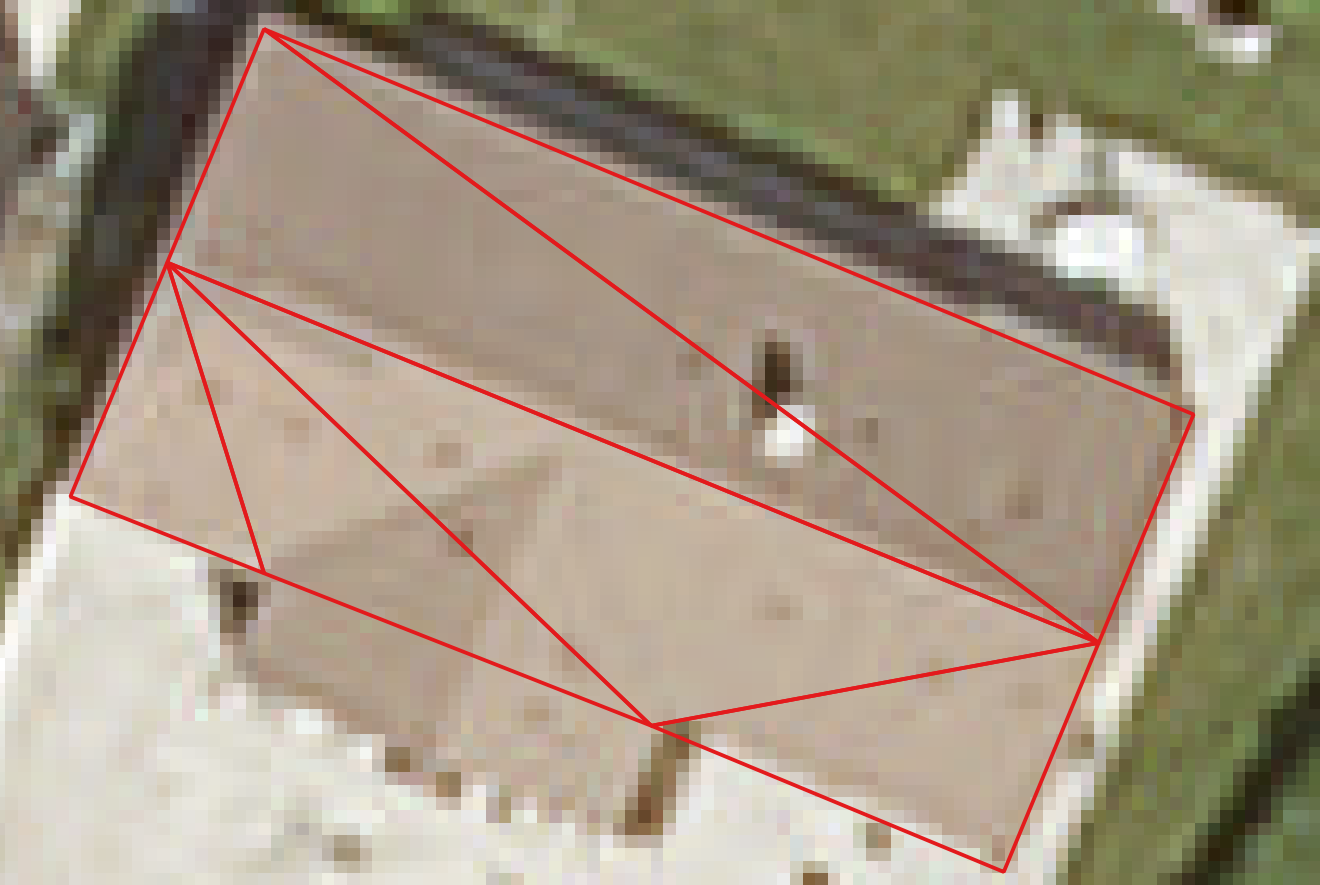
\includegraphics[width=\textwidth]{images/errors/facet/mis_segmentation}}
                                \caption{\label{fig::fac_footprint} Facet imprecise segmentation}
                            \end{subfigure}
                            \hspace{10pt}
                            \begin{subfigure}{.28\textwidth}
                                \fbox{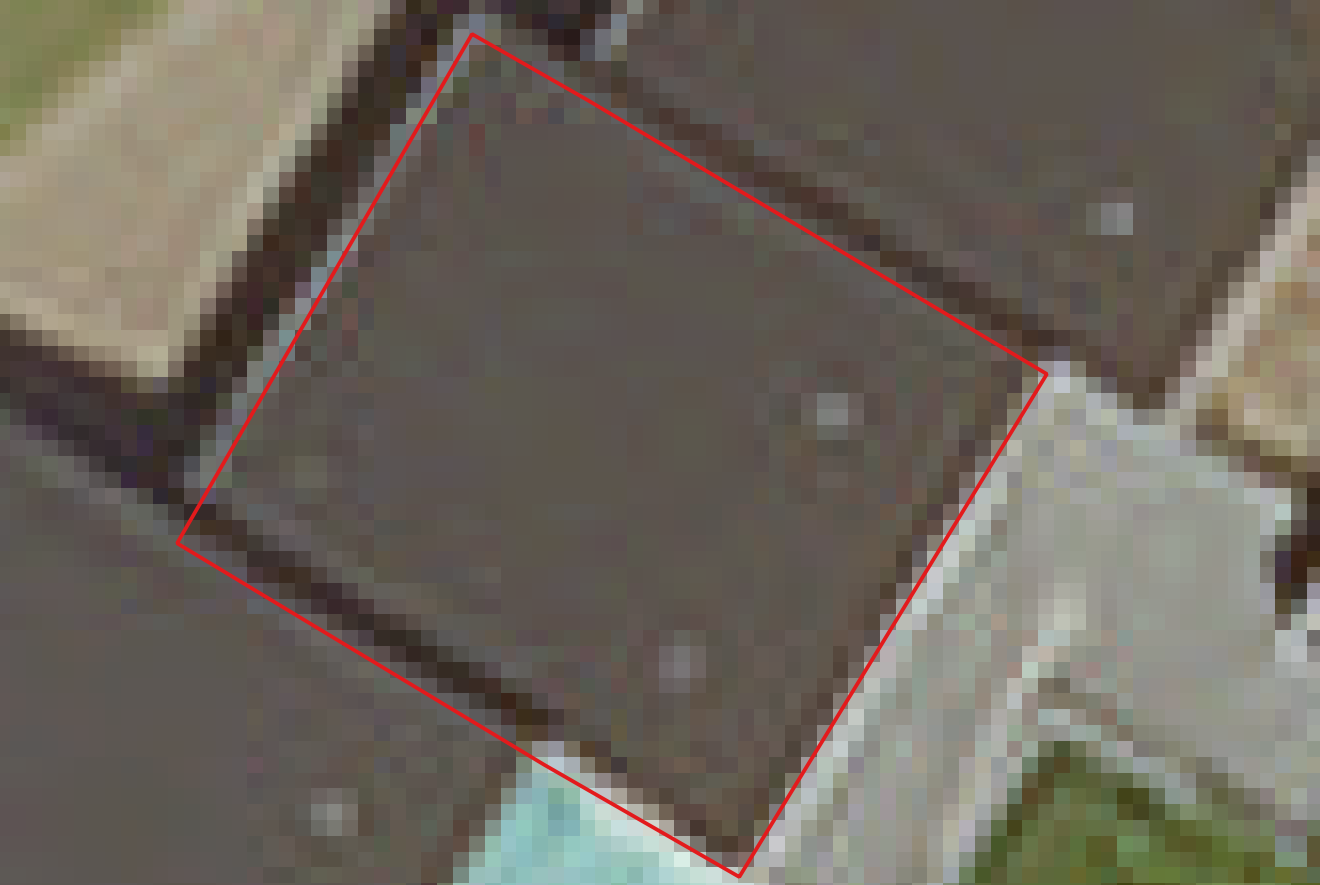
\includegraphics[width=\textwidth]{images/errors/facet/slope}}
                                \caption{\label{fig::fac_height} Imprecise height}
                            \end{subfigure}
                            \caption{Facet \emph{atomic} errors illustration.}
                        \end{center}
                    \end{figure}
                }
            \end{frame}
            \begin{frame}{Taxonomy scores}
                \begin{itemize}[label=$\blacktriangleright$, font=\color{IGNGreen}]
                    \item<1-> Each \emph{atomic} error has a score assigned to it.
                    \item<2-> The scores are from \numrange{0}{10} $\Rightarrow$ discretisation of the probability or the error occurence.
                    \item<3-> A parent error inherits the score from its child errors:
                    \begin{equation*}
                        score(p) \triangleq \max_{c \in children(p)} score(c)
                    \end{equation*}
                \end{itemize}
            \end{frame}
            \begin{frame}{Taxonomy mindmap}
                \begin{figure}
                    \includestandalone[mode=buildnew, width=\textwidth]{mind_map}
                    \caption{\label{fig::mindmap} Mindmap summarizing the error taxonomy.}
                \end{figure}
            \end{frame}
            \begin{frame}{Qualification using error taxonomy}
                The qualification has $3$ parameters:
                \begin{itemize}[label=$\blacktriangleright$, font=\color{IGNGreen}]
                    \item<1-> \emph{finesse}: the semantic level desired;
                    \item<2-> $\gls{lod}$: the diagnostic level of details. Default $ = \gls{lod}(input) $;
                    \item<3-> \emph{exclusivity}: report only the lowest \gls{lod} errors (\emph{exclusive}) or all errors (\emph{non exclusive}).
                \end{itemize}
            \end{frame}
    \section{Classification}
        \subsection{Descriptors}
            \begin{frame}{Descriptor types}
                We define a baseline for:
                \begin{enumerate}[label = (\roman*)., font=\color{black}]
                    \item<1-> Basic intrinsic descriptor:
                    \begin{itemize}[label=$\blacktriangleright$, font=\color{IGNGreen}]
                        \item<2-> \textbf{Geometric} features based on the graph $\mathscr{G}=(facets, E)$\footnote{$E \triangleq \{\text{f and g are adjacent}: (f, g) \in facets \times facets\}$};
                    \end{itemize}
                    \item<3-> Optional descriptors:
                    \begin{itemize}[label=$\blacktriangleright$, font=\color{blue}]
                        \item<4-> \textbf{Altimetric} features;
                        \item<5-> \textbf{Radiometric} features;
                    \end{itemize}
                \end{enumerate}
            \end{frame}
            \begin{frame}{Geometric features}
                \begin{equation}\label{eq::feature_vec}
                    \text{features}(m) = \begin{bmatrix}
                            S(\{\vert \{e: e \in f\} \vert : f \in facets(m)\})\\
                            S(\{\mathscr{A}(f) : f \in facets(m)\})\\
                            S(\{d(\mathscr{C}(f), \mathscr{C}(g)) : (f, g) \in facets(m)^2 \cap E(m)\})\\
                            S(\{acos(\vec{n}(f) . \vec{n}(g)) : (f, g) \in facets(m)^2 \cap E(m)\})
                    \end{bmatrix}
                \end{equation}
                \begin{itemize}
                    \only<1>{
                        \item where:
                        \begin{equation*}
                            S: x \mapsto \begin{bmatrix}
                                \max x\\
                                \min x\\
                                \overline{x}\\
                                median(x)
                            \end{bmatrix}
                        \end{equation*}
                    }
                    \only<2>{
                        \item or:
                        \begin{equation*}
                            S_{params}: x \mapsto histogram(x, params)
                        \end{equation*}
                    }
                \end{itemize}
            \end{frame}
            \begin{frame}{Altimetric features}
                \begin{equation}\label{eq::feature_vec}
                    \text{features}(m) = S_{params}(\gls{dsm} - z\ profile)
                \end{equation}
                \begin{itemize}[itemsep=5em]
                    \item where:
                    \begin{equation*}
                        S_{params}: x \mapsto histogram(x, params)
                    \end{equation*}
                    \item There is no theoretic bounds over the altimetric difference.
                    \begin{itemize}[font=\color{IGNDarkOrange}]
                        \item[$\Rightarrow$] We compute the bounds over the whole dataset in order to compute the histogram bins.
                    \end{itemize}
                \end{itemize}
            \end{frame}
            \begin{frame}{Altimetric features}
                \begin{figure}
                    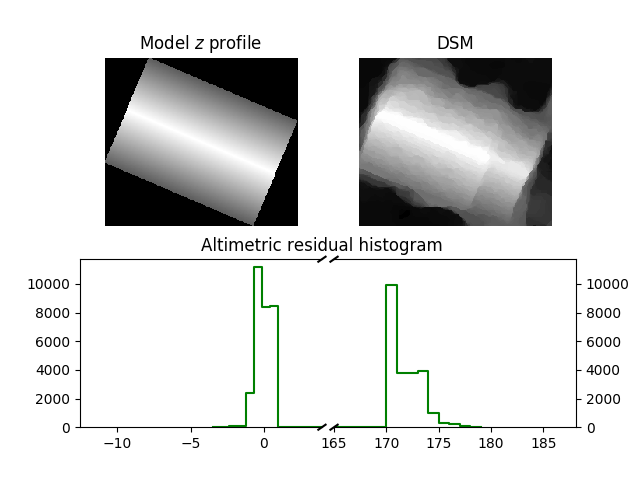
\includegraphics[height=.7\textheight]{images/altimetric_features}
                    \caption{\label{fig::altimetric} Altimetric features illustration.}
                \end{figure}
            \end{frame}
            \begin{frame}{Radiometric features}
                \begin{figure}

                    \caption{\label{fig::radiometric} Radiometric features illustration.}
                \end{figure}
            \end{frame}
            \begin{frame}{Radiometric features}
                \begin{itemize}[label=$\blacktriangleright$, font=\color{IGNGreen}]
                    \item<1-> A histogram of gardient correlation is computed along each segment:
                    \begin{multline}
                        Corr_{params}(s) = hist \Bigg( \Big\{\frac{\nabla I(p) . \vec{n}(s)}{\vert\nabla I(p)\vert}: p \in I \text{ and } p \cap s \neq \emptyset \Big\}\\
                        , params\Bigg)
                    \end{multline}
                    \item<2-> For each model $m$, we compute then:
                    \begin{equation}
                        Corr_{params}(m) = \mathscr{P}(m) . \sum_{Pol \in m} \mathscr{A}(Pol). \sum_{s \in Pol} \vert\vert s \vert\vert_2. Corr_{params}(s)
                    \end{equation}
                \end{itemize}
            \end{frame}
        \subsection{Classifiers}
            \begin{frame}{Random Forest}
                Any supervized classifier can be used in our problem. We opted for a Random Forest classifier, because:
                \begin{itemize}[label=$\blacktriangleright$, font=\color{IGNGreen}]
                    \item<1-> it handles well multimodal features;
                    \item<2-> being based on a boosting method, it is build to avoid overfitting;
                    \item<3-> it is easy to infer feature importance from.
                \end{itemize}
                \uncover<3->{
                    We choose:
                    \begin{itemize}[label=$\blacktriangleright$, font=\color{IGNGreen}]
                        \item<4-> $4$ maximum depth to avoid overfitting the trees;
                        \item<5-> $800$ trees to cover the whole the attributes space.
                    \end{itemize}
                }
            \end{frame}
            \begin{frame}{Multi-Class, Multi-Label or Multi-Stage}
                \begin{itemize}[label=$\blacktriangleright$, font=\color{IGNGreen}]
                    \item<1-> Depending on the \emph{finesse} and the \emph{exclusivity} parameters, we get:
                    \begin{itemize}[label=--]
                        \item<2-> \textbf{Multi-Class}: one label to predict, multiple cases to predict;
                        \item<3-> \textbf{Multi-Label}: multiple labels to predict, each has multiple cases (in our case, \textbf{binary});
                        \item<3-> \textbf{Multi-Stage} or Hierchical: one \textbf{Multi-Class} stage to predict the \emph{error family} and then a \textbf{Multi-Label} one to detect the corresponding \emph{atomic} errors.
                    \end{itemize}
                    \item<4-> We adapt any \textbf{Multi-Class} or \textbf{binary} classifier to be the \textbf{Multi-Label} setting using a \emph{OnevsAll} strategy.
                \end{itemize}
            \end{frame}
        \subsection{Results}
            \begin{frame}{Used Data}
                \begin{itemize}[leftmargin=6em, font=\color{IGNDarkGreen}]
                    \item[Town:]<1-> Elancourt (Yvelines, France);
                    \item[Area:]<2-> \SI{0.2}{\km \squared};
                    \item[Buildings:]<3-> $502$;
                    \item[Type:]<4-> mostly residential district with a school and one gas station;
                    \item[Algorithm:]<5-> $\text{Bati3D}^\text{\textregistered}$~\footfullcite{Durupt2006}.
                \end{itemize}
            \end{frame}
            \begin{frame}{Ground truth statistics}
                \begin{table}
                    \tiny
                    \begin{center}
                        \begin{tabular}{|x{2cm} | x{1.2cm} | x{2cm} | x{1.5cm} | x{1.5cm}|}
                            \hline
                            \multicolumn{1}{|c|}{\textbf{Error Class}} & \textbf{Occurence ratio} & \textbf{\emph{Atomic} error} & \textbf{Family conditionnal occurence ratio} & \textbf{Absolute occurence ratio} \\
                            \hline
                            Unqualifiable & $0.0876$ & -- & -- & -- \\
                            \hline
                            \hline
                            \multirow{4}{*}{Building Errors} & \multirow{4}{*}{$0.2408$} & Over segmentation & $0.1365$ & $0.0328$\\
                            \cline{3-5}
                                &                   & Under segmentation & $0.4177$ & $0.1006$ \\
                            \cline{3-5}
                                &                   & Imprecise footprint & $0.4839$ & $0.1165$ \\
                            \cline{3-5}
                                &                   & Imprecise height & $0.0165$ & $0.0040$ \\
                            \hline
                            \hline
                            \multirow{4}{*}{Facet Errors} & \multirow{4}{*}{$0.81657$} & Over segmentation & $0.8830$ & $0.7203$ \\
                            \cline{3-5}
                                &                   & Under segmentation & $0.0842$ & $0.0687$ \\
                            \cline{3-5}
                                &                   & Imprecise segmentation & $0.0806$ & $0.0657$ \\
                            \cline{3-5}
                                &                   & Imprecise slope & $0.0327$ & $0.0267$ \\
                            \hline
                        \end{tabular}
                        \caption{\label{tab::label_stats} Label statistics over the dataset.}
                    \end{center}
                \end{table}
            \end{frame}
            \begin{frame}{Results}
                \begin{table}
                    \begin{subtable}{.4\textwidth}
                        \tiny
                        \begin{center}
                            \begin{tabular}{x{1cm} x{.5cm} x{.5cm} x{.5cm}}
                                \toprule
                                {\bf Error} & {\bf OA} & {\bf Recall} & {\bf Precision} \\
                                \midrule
                                Building Errors & $0.81$ & $0.39$ & $0.76$ \\
                                \midrule
                                Facet Errors & $0.92$ & $0.97$ & $0.93$ \\
                                \bottomrule
                            \end{tabular}
                            \caption{\tiny\label{tab::finesse2} $finesse = 2$}
                        \end{center}
                    \end{subtable}
                    \begin{subtable}{.45\textwidth}
                        \tiny
                        \begin{center}
                            \begin{tabular}{x{1.75cm} x{.5cm} x{.5cm} x{.5cm}}
                                \toprule
                                {\bf Error} & {\bf OA} & {\bf Recall} & {\bf Precision} \\
                                \midrule
                                Buil. Under Seg. & $0.95$ & $0.63$ & $0.87$ \\
                                \midrule
                                Buil. Over Seg. & $0.97$ & $0.16$ & $1.0$ \\
                                \midrule
                                Footprint & $0.91$ & $0.24$ & $0.93$ \\
                                \midrule
                                Height & $0.99$ & $0.0$ & --- \\
                                \midrule
                                \midrule
                                Fac. Under Seg. & $0.92$ & $0.14$ & $0.41$ \\
                                \midrule
                                Fac. Over Seg. & $0.99$ & $1.0$ & $0.99$ \\
                                \midrule
                                Fac. Impr. Seg. & $0.92$ & $0.0$ & ---\\
                                \midrule
                                Slope & $0.97$ & $0.14$ & $1.0$\\
                                \bottomrule
                            \end{tabular}
                            \caption{\tiny\label{tab::finesse3}$finesse = 3$}
                        \end{center}
                    \end{subtable}
                    \caption{Test results for a \emph{non exclusive} qualification with $\gls{lod}=2$ using a $10- fold$ classification.}
                \end{table}
            \end{frame}
            \begin{frame}{Discussion}
                \begin{itemize}[label=$\blacktriangleright$, font=\color{IGNGreen}]
                    \item<1-> Unbalanced \textbf{Building Errors} ($24\%$ among the $502$ instances) $\Rightarrow$ small recall.
                    \item<2-> Among the \textbf{Facet Errors}, all but \textbf{Facet Over segmentation} suffer from the unbalanced dataset (ratio $ < 7\%$) $\Rightarrow$ small recall and big overall accuracy.
                    \item<3-> Geometric features alone can predict errors with a comparable order of accuracy.
                \end{itemize}
            \end{frame}
    \section{Perspectives}
        \subsection{Data augmentation}
            \begin{frame}{The need for more data}
                We need more data:
                \begin{itemize}[label=$\blacktriangleright$, font=\color{IGNGreen}]
                    \item to have enough representative samples for each error for the learning step;
                    \item to avoid overfitting to a specific urban scene or a specific reconstruction method.
                \end{itemize}
            \end{frame}
            \begin{frame}{More annotations}
                \begin{itemize}[label=$\blacktriangleright$, font=\color{IGNGreen}]
                    \item<1-> One difficult aspect of the methodology is the annotation phase.
                    \item<2-> A Master's (PPMD) student made a \emph{QT5} \acrshort{gui} python application. It can be used:
                    \begin{itemize}[label=--]
                        \item<3-> for annotation purposes,
                        \item<4-> for prediction verification,
                        \item<5-> in a semi-automatic learning pipeline.
                    \end{itemize}
                    \item<6-> We can also consider error simulation using a reference data.
                \end{itemize}
            \end{frame}
            \begin{frame}{More scenes}
                \begin{itemize}[label=$\blacktriangleright$, font=\color{IGNGreen}]
                    \item<1-> We need to procure more reconstructed scenes using $\text{Bati3D}^\text{\textregistered}$.
                    \item<2-> A group of students (ENSG) reconstructed Elancourt and Toulouse using the \emph{3dfier} program~\footfullcite{ledoux2011topologically}: $\gls{lod} = 1$;
                    \item<3-> We can compare with other reconstruction methods~\footfullcite{Lafarge2012,kelly2017bigsur}.
                \end{itemize}
            \end{frame}
        \subsection{Unsupervized learning}
            \begin{frame}{Unsupervized learning}
                We consider exploring unsupervized learning, to:
                \begin{itemize}[label=$\blacktriangleright$, font=\color{IGNGreen}]
                    \item discover errors not categorized in our taxonomy;
                    \item scale learned classifiers over other scenes.
                \end{itemize}
            \end{frame}
        \subsection{Learned features}
            \begin{frame}{Graph kernels \& Deep learning}
                We consider investigating:
                \begin{itemize}[label=$\blacktriangleright$, font=\color{IGNGreen}]
                    \item<1-> Graph kernels:
                    \begin{itemize}
                        \item[\color{green} +]<2-> it can be feasible: we mostly have small graphs.
                        \item[\color{green} +]<3-> it takes advantage of the model structure better than simple histograms;
                        \item[\color{red} --]<4-> it requires high computational capacity.
                    \end{itemize}
                    \item<5-> Deep learning:
                    \begin{itemize}
                        \item[\color{green} +]<6-> its capacity has been proven for images;
                        \item[\color{green} +]<7-> it is highly semantic and transferable;
                        \item[\color{red} --]<8-> it requires a big number of instances.
                    \end{itemize}
                \end{itemize}
            \end{frame}
    \section{Conclusion}
        \begin{frame}{Conclusion}
            \begin{itemize}
                \item We propose a new qualification framework for building $3D$ polyhedric models;
                \item We categorize $3D$ model errors into a flexible taxonomy independent from the reconstruction method;
                \item We propose a flexible and modular classification pipeline using supervised learning;
                \item We established a baseline for geometric, radiometric and altimetric features.
            \end{itemize}
        \end{frame}
    \section*{References}
        \begin{frame}[allowframebreaks]{References}
            \printbibliography
        \end{frame}
\end{document}
